\section{Цель работы}
Изучение инструментальных средств идентификации объектов управления

\section{Задачи}

\begin{itemize}
	\item построение линейной компьютерной модели, идентификация модели методом подстраиваемых параметров;
	\item построение компьютерной модели объекта управления с учетом нелинейности объекта, идентификация модели методом подстраиваемых параметров;
	\item построение нейросетевой модели объекта управления.
\end{itemize}

\section{Основные теоретические положения}
Первоочередной задачей при разработке системы управления является получение модели объекта управления. Существует два способа построения модели объекта: аналитический и экспериментальный. В случае аналитического способа имеются априорные знания о законах природы, которым подчиняются процессы, что позволяет описать объект без проведения экспериментов. В случае «серого» ящика о внутренней структуре объекта известна некоторая информация, но ее недостаточно для построения модели. Тогда применяют экспериментальный способ, который заключается в подаче тестовых сигналов на вход объекта, анализе реакций и обработке данных. На практике комбинируют аналитический и экспериментальный способы

Способы идентификации далее рассмотрены без объяснения методов и алгоритмов обработки данных, которые детально изучаются в рамках дисциплины «Идентификация объектов управления». Существенным упрощением работы является отсутствие случайных возмущений. Это исключает необходимость в многократных экспериментах, хотя не вполне соответствует понятию и термину «идентификация»

Рассматриваются компьютерные имитаторы объектов с одним входом и одним выходом (типа SISO)

Если точный вид нелинейности является неизвестным и нетиповым, то можно воспользоваться универсальной моделью на базе искусственных нейронных сетей. Процедура идентификации, т. е. подстройка параметров сети мало отличается от заданной исследователем типовой модели, однако, как правило, используются более сложные методы оптимизации в силу большего числа параметров

Изначально идея нейросетевых моделей пришла из биологии на основе биологического нейрона, однако искусственные нейронные сети имеют общего с биологическими только название. Если опустить вопросы связанные с обучением и специфическими архитектурами, то нейронные сети можно представить, как различного рода соединения искусственных нейронов, являющиеся взвешенным сумматором и описываемых следующими формулами:
$$
y = f(u) \\
u = \sum_{i=1}^{n}  \omega_i x_i + \omega_0 x_0
$$

Где $x_i$ - сигнал на входе нейрона, $\omega_i$ - вес соответствующего входа, $\omega_0, x_0$ дополнительный инициализирующий вход и его вес, обеспечивающий постоянное смещение. $f(u)$ - функция активации, которой может являться одна из множества линейных или нелинейных функций

\section{Обработка результатов эксперимента}

\subsection{Свободные движения объекта}
Проверим работу модели построим свободные движения системы (движения с нулевым входом) (Рис. \ref{fig:1}).

\begin{figure}[H]
	\centering
	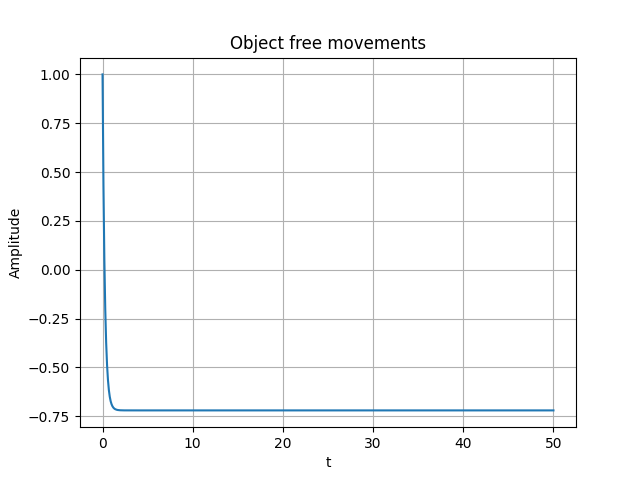
\includegraphics[width=0.9\linewidth]{body/images/Object-free-movements.png}
	\caption{Свободные движения объекта}
	\label{fig:1}
\end{figure}

Данный график напоминает график ПФ апериодического звена первого порядка. Можно отметить достаточно долгий переходный процесс,
и, следовательно, большую постоянную времени звена

\subsection{Проведение эксперимента}
Для анализа поведения объекта исследуем отклик при подаче различных тестовых воздействий:
\begin{itemize}
	\item моногармонический сигнал
	\item импульсное воздействие длиной 0.01
	\item нормированное импульсное воздействие длиной 0.01
	\item меандр
	\item ступенчатое воздействие
\end{itemize}

\subsubsection{Моногармонический сигнал}
Рассмотрим реакцию системы на моногармонический сигнал (Рис. \ref{fig:2}).

\begin{figure}[H]
	\centering
	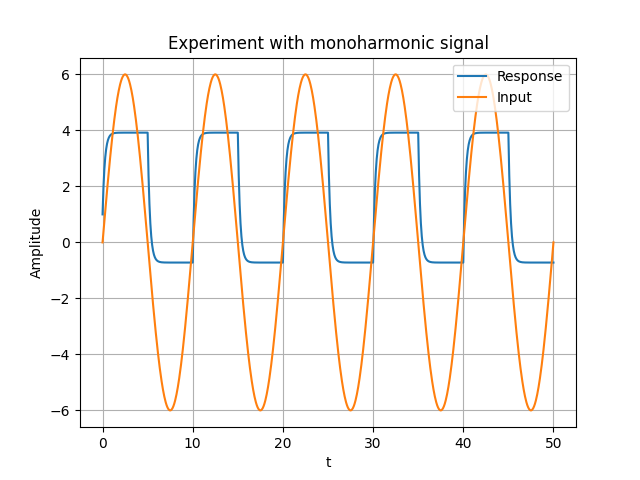
\includegraphics[width=0.9\linewidth]{body/images/Experiment-with-monoharmonic-signal.png}
	\caption{Моногармонический сигнал и реакция системы на него же}
	\label{fig:2}
\end{figure}

Предположим, что в системе присутствует апериодическое звено первого порядка. Сравним отклик данного звена с параметрами $ k = 1, T = 0.5 $ на моногармонический сигнал с откликом системы (Рис. \ref{fig:3})

\begin{figure}[H]
	\centering
	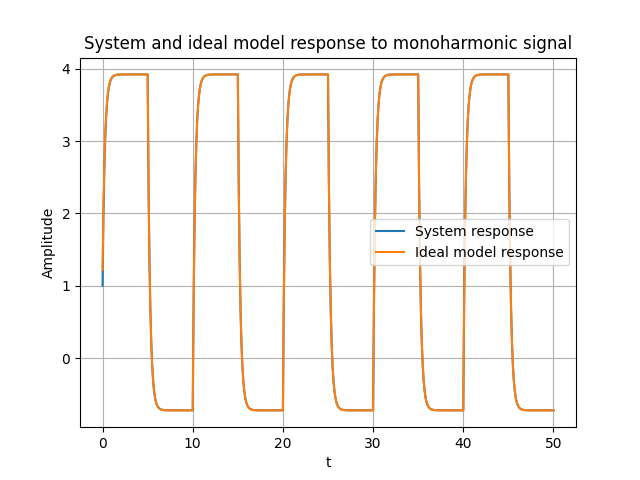
\includegraphics[width=0.9\linewidth]{body/images/System-and-ideal-model-response-to-monoharmonic-signal.png}
	\caption{Реакция системы на моногармонический сигнал и реакция линейного звена на него же}
	\label{fig:3}
\end{figure}

Откорректированные значения, полученные программно с помощью способа наименьших квадратов:

$Estimated\quad parameter:$

\qquad$[0.498997\quad 0.391651]$

$Estimated\quad initial\quad condition: [4.401772]$

Из графика (Рис. \ref{fig:3}) следует, что линейного звена недостаточно, чтобы полностью воспроизвести отклик системы

Рассмотрев графики реакции системы на моногармонический сигнал и реакцию линейного звена на него же, можно убедиться в том,
что в системе присутствует и нелинейность: "Идеальное реле". Параметры нелинейности "Идеальное реле", навскидку, примем $ c_1 = 4, c_2 = 0.7 $. Линейные параметры оставим без изменений

\begin{figure}[H]
	\centering
	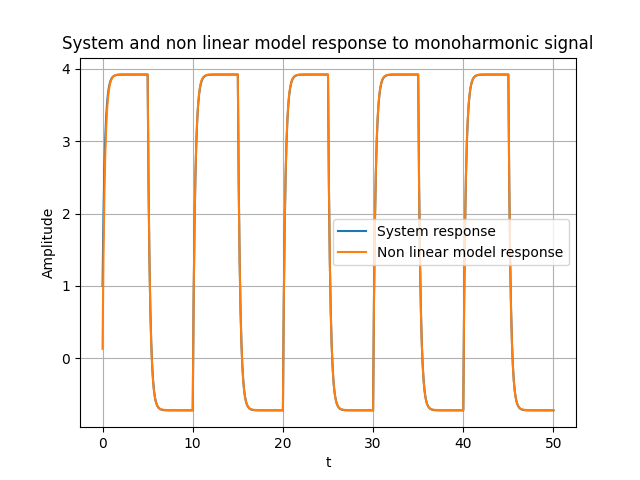
\includegraphics[width=0.9\linewidth]{body/images/System-and-non-linear-model-response-to-monoharmonic-signal.png}
	\caption{Реакция системы на моногармонический сигнал и реакция нелинейного звена на него же}
	\label{fig:4}
\end{figure}

Откорректированные значения, полученные программно с помощью способа наименьших квадратов:

$Estimated\quad parameter:$

\qquad$[0.917059\quad 0.245550\quad 4.277298886363543\quad 0.780468]$

$Estimated\quad initial\quad condition: [0.131380]$

Моногармонический сигнал отлично отражает то, что в системе присутствует нелинейность. Как и предпологалось, эта нелинейность - "Идеальное реле".
На графике (Рис. \ref{fig:4}) очень хорошо видно приведение моногармонического сигнала к типовому виду меандра. Амплитуды выше нуля ставновятся равными
нелинейному параметру, навскидку оценённому как $ c_1 = 4 $, нелинейности "Идеальное реле". Ниже нуля ситуация такая же: всё приводится к нелинейному параметру, навскидку оценённому как $ c_2 = 0.7 $.
Помимо этого, предположения насчёт типа нелинейности подтверждает и почти полное совпадение реакции системы и реакции нелинейного звена

Примем данные параметры во внимание при следующих экспериментах

Примем, что искомая нелинейность - "Идеальное реле"

\subsubsection{Импульсное воздействие}
Рассмотрим реакцию системы на импульсное воздействие (Рис. \ref{fig:5})

\begin{figure}[H]
	\centering
	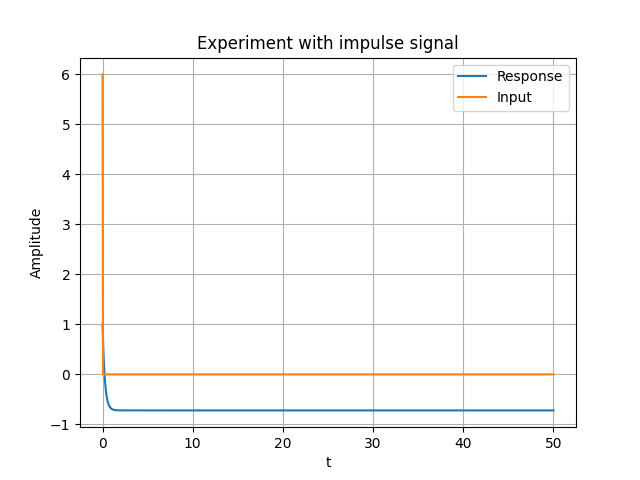
\includegraphics[width=0.8\linewidth]{body/images/Experiment-with-impulse-signal.png}
	\caption{Импульсное воздействие и реакция системы на него же}
	\label{fig:5}
\end{figure}

На этом графике уже лучше видно, что затухание происходит очень быстро. Примем параметрамы $ k = 1, T = 0.5 $

\begin{figure}[H]
	\centering
	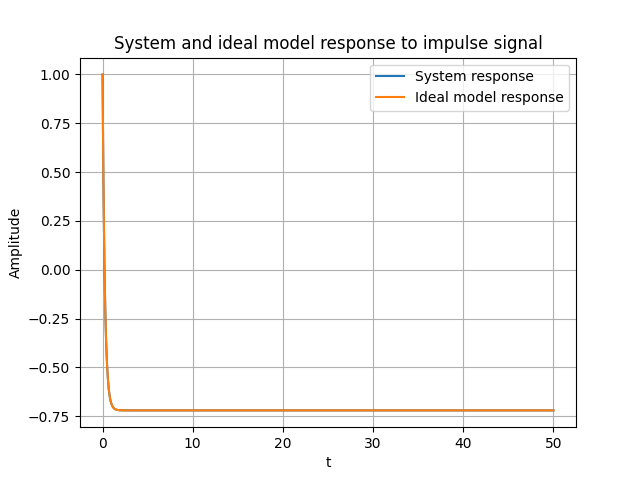
\includegraphics[width=0.8\linewidth]{body/images/System-and-ideal-model-response-to-impulse-signal.png}
	\caption{Реакция системы на импульсное воздействие и реакция линейного звена на него же}
	\label{fig:6}
\end{figure}

Откорректированные значения, полученные программно с помощью способа наименьших квадратов:

$Estimated\quad parameter:$

\qquad$[1.0\quad 0.5]$

$Estimated\quad initial\quad condition: [1.666e-08]$

Даже по оценке линейных параметров видно непоказательность импульсного воздействия. Предположить тип нелинейности здесь тоже очень трудно.
Сами же параметры остаются такими, меняется только лишь начальное условие, что подтверждает описанное выше

Из графика (Рис. \ref{fig:6}) следует, что линейного звена недостаточно, чтобы полностью воспроизвести отклик системы

Примем параметры нелинейности "Идеальное реле", как и прошлом эксперименте: $ c_1 = 4, c_2 = 0.7 $. Линейные параметры оставим без изменений


\begin{figure}[H]
	\centering
	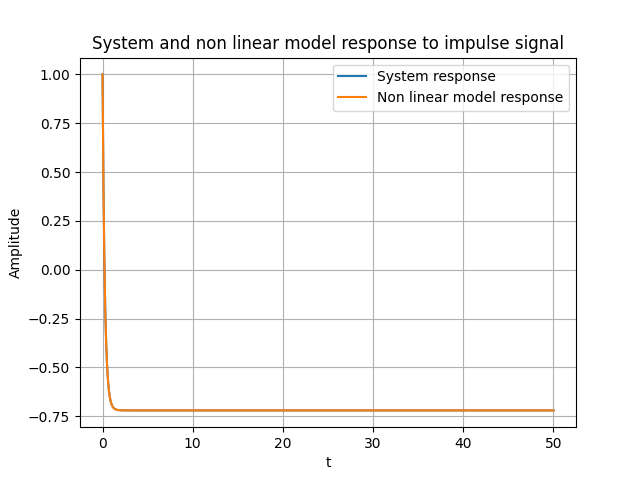
\includegraphics[width=0.8\linewidth]{body/images/System-and-non-linear-model-response-to-impulse-signal.png}
	\caption{Реакция системы на импульсное воздействие и реакция нелинейного звена на него же}
	\label{fig:7}
\end{figure}

Откорректированные значения, полученные программно с помощью способа наименьших квадратов:

$Estimated\quad parameter:$

\qquad$[0.998197\quad 0.250000\quad 3.737908\quad 0.721300]$

$Estimated\quad initial\quad condition: [0.999999]$

На графике (Рис. \ref{fig:7}) не видно приведение импульсного воздействия к типовому виду меандра практические никак

\subsubsection{Нормированное импульсное воздействие}
Рассмотрим реакцию системы на нормированное импульсное воздействие (Рис. \ref{fig:8})

\begin{figure}[H]
	\centering
	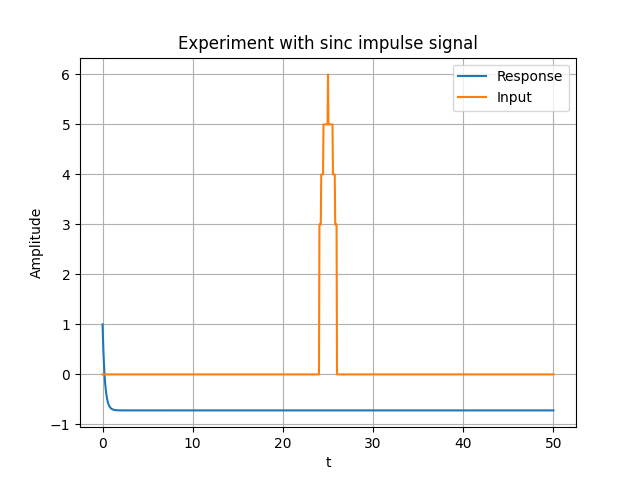
\includegraphics[width=0.7\linewidth]{body/images/Experiment-with-sinc-impulse-signal.png}
	\caption{Импульсное воздействие и реакция системы на него же}
	\label{fig:8}
\end{figure}

На этом графике, как и на графике для импульсного воздействия, видно, что затухание происходит очень быстро. Примем параметрамы $ k = 1, T = 0.5 $

\begin{figure}[H]
	\centering
	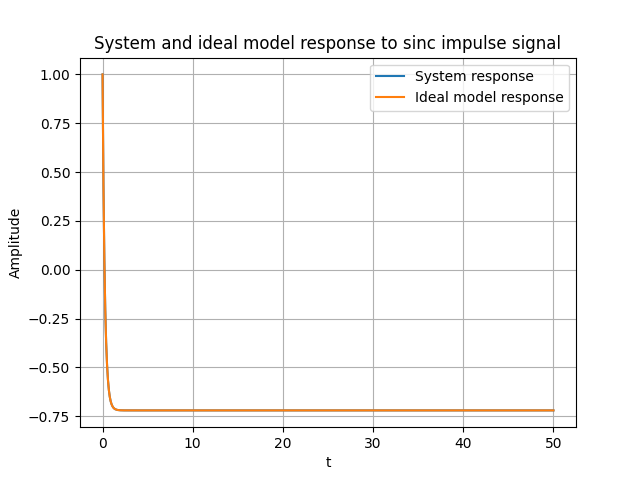
\includegraphics[width=0.7\linewidth]{body/images/System-and-ideal-model-response-to-sinc-impulse-signal.png}
	\caption{Реакция системы на нормированное импульсное воздействие и реакция линейного звена на него же}
	\label{fig:9}
\end{figure}

Откорректированные значения, полученные программно с помощью способа наименьших квадратов:

$Estimated\quad parameter:$

\qquad$[1.0\quad 1.184270]$

$Estimated\quad initial\quad condition: [-0.440800]$

Здесь уже немного видны изменения по сравнению с обычным импульсным воздействием. Предположить тип нелинейности по-прежнему затруднительно в следствие непоказательности.

Из графика (Рис. \ref{fig:9}) следует, что линейного звена недостаточно, чтобы полностью воспроизвести отклик системы

Примем параметры нелинейности "Идеальное реле", как и прошлом эксперименте: $ c_1 = 4, c_2 = 0.7 $. Линейные параметры оставим без изменений

\begin{figure}[H]
	\centering
	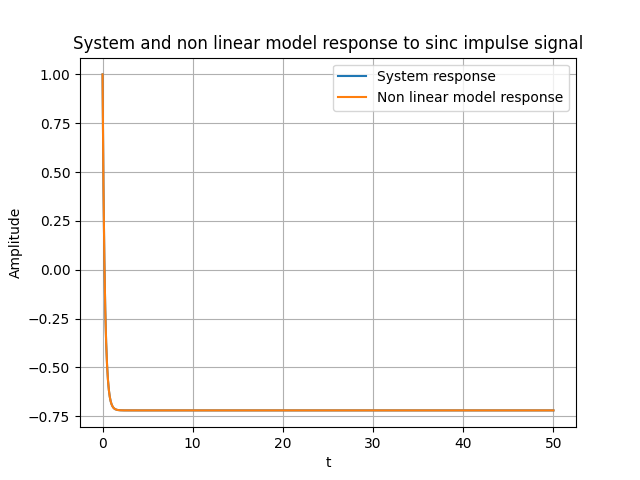
\includegraphics[width=0.9\linewidth]{body/images/System-and-non-linear-model-response-to-sinc-impulse-signal.png}
	\caption{Реакция системы на нормированное импульсное воздействие и реакция нелинейного звена на него же}
	\label{fig:10}
\end{figure}

Откорректированные значения, полученные программно с помощью способа наименьших квадратов:

$Estimated\quad parameter:$

\qquad$[1.0008193742168756\quad 0.25000000004563155\quad 3.9999985883519122\quad 0.7194105357599472]$

$Estimated\quad initial\quad condition: [1.0000000000098128]$

На графике (Рис. \ref{fig:10}) не видно приведение нормированного импульсного воздействия к типовому виду меандра

\subsubsection{Меандр}
Рассмотрим реакцию системы на меандр (Рис. \ref{fig:11})

\begin{figure}[H]
	\centering
	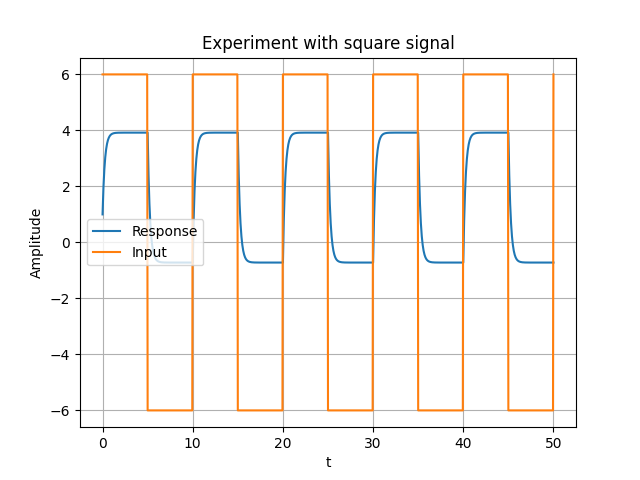
\includegraphics[width=0.7\linewidth]{body/images/Experiment-with-square-signal.png}
	\caption{Меандр и реакция системы на него же}
	\label{fig:11}
\end{figure}

Уже даже сейчас мы можем сказать, что нелинейность, определённая в первом эксперименте, точно является нелинейностью "Идеальное реле". Примем те же параметры $ k = 1, T = 0.5 $

\begin{figure}[H]
	\centering
	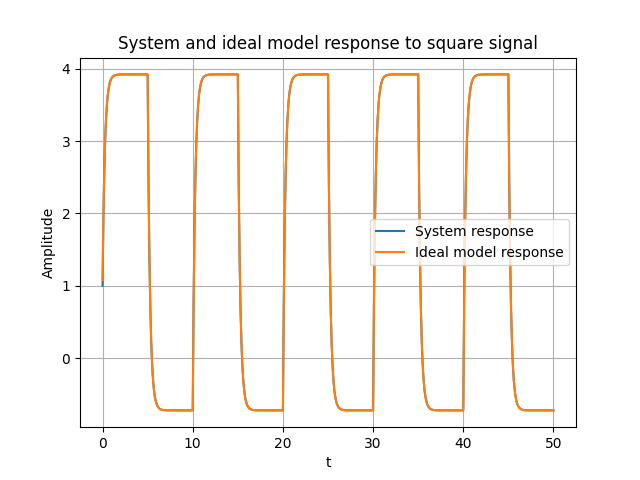
\includegraphics[width=0.7\linewidth]{body/images/System-and-ideal-model-response-to-square-signal.png}
	\caption{Реакция системы на меандр и реакция линейного звена на него же}
	\label{fig:12}
\end{figure}

Откорректированные значения, полученные программно с помощью способа наименьших квадратов:

$Estimated\quad parameter:$

\qquad$[0.388511\quad 0.284591]$

$Estimated\quad initial\quad condition: [0.705437]$

Из рисунка (Рис. \ref{fig:12}) становится ясно, что даже линейной модели достаточно, чтобы смоделировать реакцию системы. Остаётся только сместить отклик по амплитуде.
Предположительная идентичность и достаточность линейной модели объясняется тем, что исходный сигнал является меандром, а нелинейность "Идеальное реле" преобразует сигнал в меандр,
верхняя и нижняя амплитуды которого регулируются усилением и нелинейными параметрами

Примем параметры нелинейности "Идеальное реле", как и всех прошлых экспериментах: $ c_1 = 4, c_2 = 0.7 $. Линейные параметры оставим без изменений

\begin{figure}[H]
	\centering
	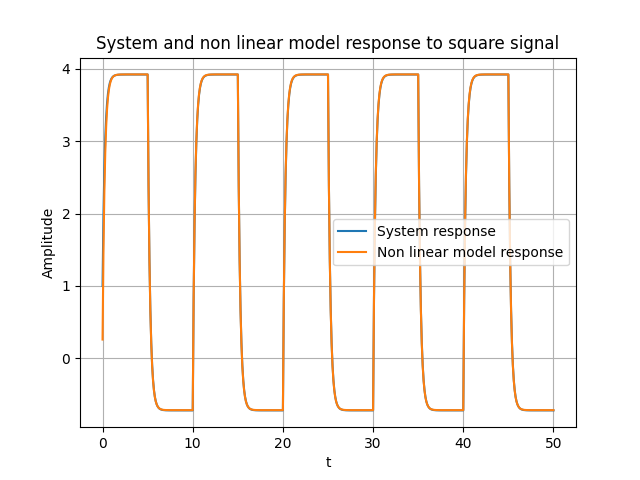
\includegraphics[width=1\linewidth]{body/images/System-and-non-linear-model-response-to-square-signal.png}
	\caption{Реакция системы на меандр и реакция нелинейного звена на него же}
	\label{fig:13}
\end{figure}

Откорректированные значения, полученные программно с помощью способа наименьших квадратов:

$Estimated\quad parameter:$

\qquad$[1.000382\quad 0.246545\quad 3.920302\quad 0.716238]$

$Estimated\quad initial\quad condition: [0.258909]$

Заметим, что полученные оценённые параметры практически полностью, за исключением начального состояния, повторяют параметры входного нормированного импульсного воздейтсвия. Это означает,
что с точки зрения машинных средств обработки они очень схожи, а на глаз в них тяжело принять что-то схожее

Из графика (Рис. \ref{fig:13}) видно, что полученный отклик практически идеально, а если и не так, то очень схоже моделирует отклик системы. Как уже говорилось выше: это объясняется почти полным
сходством исходного сигнала и отклика нелинейности "Идеальное реле"

\subsubsection{Ступенчатое воздействие}
Рассмотрим реакцию системы на ступенчатое воздействие (Рис. \ref{fig:14})

\begin{figure}[H]
	\centering
	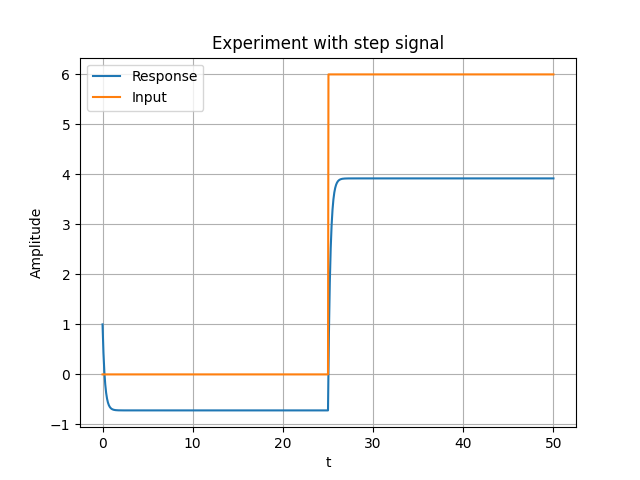
\includegraphics[width=1\linewidth]{body/images/Experiment-with-step-signal.png}
	\caption{Ступенчатое воздействие и реакция системы на него же}
	\label{fig:14}
\end{figure}

Здесь снова подтверждается, что нелинейность, определённая в первом эксперименте, точно является нелинейностью "Идеальное реле". Это и логично, так как ступенчатое воздействие - это
частый случай меандра: меандр с огромной скважностью. Примем те же линейные параметры $ k = 1, T = 0.5 $

\begin{figure}[H]
	\centering
	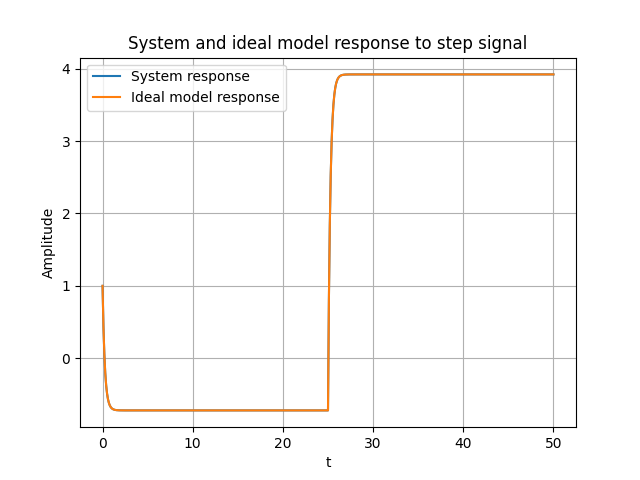
\includegraphics[width=1\linewidth]{body/images/System-and-ideal-model-response-to-step-signal.png}
	\caption{Реакция системы на ступенчатое воздействие и реакция линейного звена на него же}
	\label{fig:15}
\end{figure}

Откорректированные значения, полученные программно с помощью способа наименьших квадратов:

$Estimated\quad parameter:$

\qquad$[0.653665\quad 0.296811]$

$Estimated\quad initial\quad condition: [0.024534]$

Опять, же, из-за явления частного случая меандра повторяются и все выводы, описанные для меандра

Примем параметры нелинейности "Идеальное реле", как и прошлом эксперименте: $ c_1 = 4, c_2 = 0.7 $. Линейные параметры оставим без изменений

\begin{figure}[H]
	\centering
	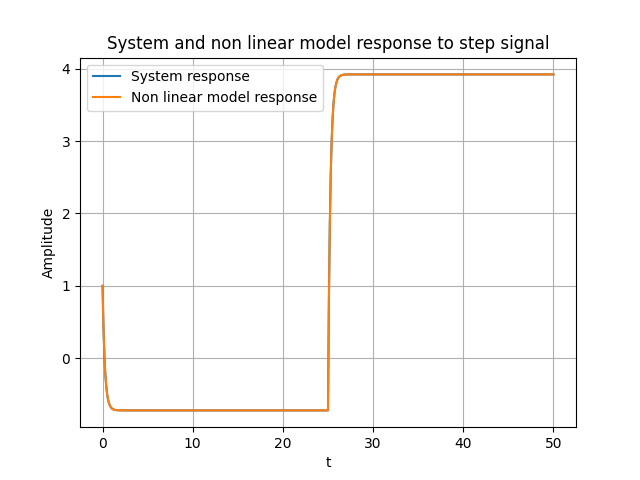
\includegraphics[width=1\linewidth]{body/images/System-and-non-linear-model-response-to-step-signal.png}
	\caption{Реакция системы на ступенчатое воздействие и реакция нелинейного звена на него же}
	\label{fig:16}
\end{figure}

Откорректированные значения, полученные программно с помощью способа наименьших квадратов:

$Estimated\quad parameter:$

\qquad$[0.9084036268803937\quad 0.25000002780572106\quad 4.315262386526328\quad 0.7925992078208546]$

$Estimated\quad initial\quad condition: [0.999999172403585]$

На графике (Рис. \ref{fig:15}) явно видна схожесть отклика нелинейного звена на ступенчатое воздействия и отклика системы на него же

\subsection{Нейросетевая модель}

Смоделируем с помощью нейросетевой модели каждый из использовавшихся в работе сигналов

Разделять выборку будем иным способом, чем в примере. Предложенный в примере способ будет не очень эффективен для таким сигналов, как импульсное, нормированное импульсное и ступенчатое воздействие.
Для тестирования выбираются конечные 30\% значений массива датасета сигнала. Для любого из импульсных воздействием мы рискуем попасть в установившийся режим,
который не будет показывать ничего, а только мешать выборке, образуя константную прямую. В случае ступенчатого воздействия всё ещё хуже: шанс попасть в константную ещё выше
из-за типовой формы сигнала. В случае использования периодических сигналов этот способ, безусловно, хорош. Особенно он хорош своей простотой понимания, вдобавок и простотой реализации

В ходе тестирования работы нейросетевой модели было принято решение о смене формата обучения и тестирования сети. Разделим выборку по простейшему золотому сечению: 2:1. Пусть две трети значений будут
для обучения сети, а оставшаяся одна треть будет валидационными значениями. Для решения проблемы с непериодическими сигналами, в нашем случае с импульсными и ступенчатым, будет делить
массив значений датасета на тройки значения. Другими словами, будем выбирать каждое 3-е значения для валидации, а оставшийся массив будем использовать непосредственно для тренировки нейросети

Реализовав алгоритм обучения и тестирования попробуем провести через нейросеть исходные сигналы

\subsubsection{Моногармонический сигнал}

\begin{figure}[H]
	\centering
	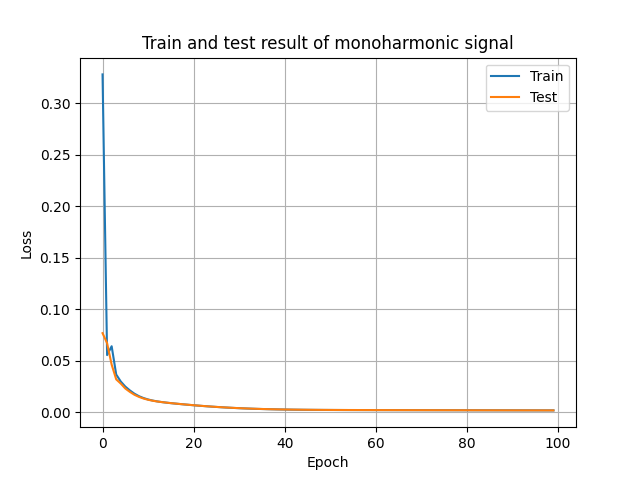
\includegraphics[width=1\linewidth]{body/images/Train-and-test-result-of-monoharmonic-signal.png}
	\caption{Отклонение значений при тренировке и тестирования нейросети, обученной на моногармоническом сигнале}
	\label{fig:17}
\end{figure}

Вы видим график (Рис. \ref{fig:17}), схожий с обратной пропорциональностью, который очень быстро опадает. Здесь явно видно, как хорошо
модель обучается: нет никаких посторонних пиков. Скорость спада графика знаменует собой крайней успешной и быстрое обучение.
На рассматриваемом промежутке в 100 эпох видно, что нейросеть не имеет уже практически никаких отклонений к 50 эпохе.
Так происходит из-за периодичности моногармонического сигнала, одинаковой амплитуды каждого лепестка

\begin{figure}[H]
	\centering
	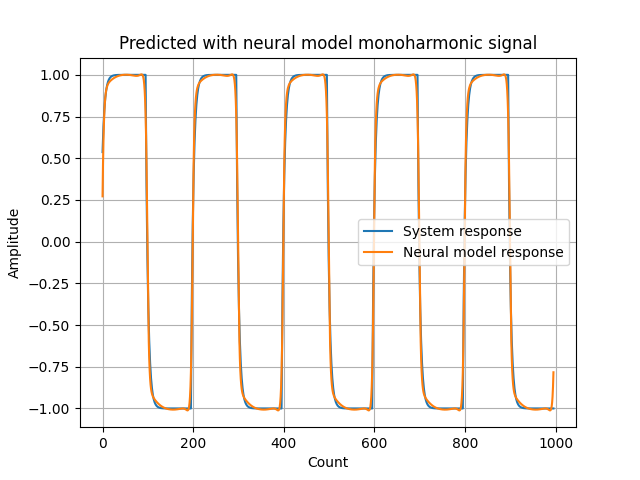
\includegraphics[width=1\linewidth]{body/images/Predicted-with-neural-model-monoharmonic-signal.png}
	\caption{Отклик системы и смоделированный отклик нейросети, обученной на моногармоническом сигнале}
	\label{fig:18}
\end{figure}

На графике (Рис. \ref{fig:18}) явно видно почти полное совпадение отклика системы на моногармонический сигнал и смоделированного нейросетевой
моделью отклика. Как и было отмечено выше, такая модель имеет склонность к быстрому обучения и меньшим тратам производительных ресурсов, следующих из предыдущего

\subsubsection{Импульсное воздействие}

\begin{figure}[H]
	\centering
	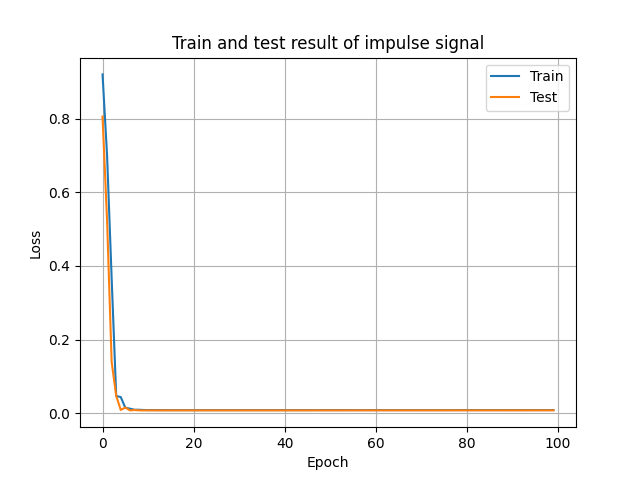
\includegraphics[width=1\linewidth]{body/images/Train-and-test-result-of-impulse-signal.png}
	\caption{Отклонение значений при тренировке и тестирования нейросети, обученной на импульсном воздействии}
	\label{fig:19}
\end{figure}

Мы видим график (Рис. \ref{fig:19}), схожий с обратной пропорциональностью, который опадает невероятно быстро.
На этом графике видны остаточные следы обучения модели: видные небольшие лепестки сразу же после падения.
Это вызвано тем, что импульсный сигнал в нашем случае находится в нуле, а значит и модель, сравнивающая значения увидит это изменение
в начальных эпохах, после чего это изменение будет ничем, превращаясь в константную прямую

\begin{figure}[H]
	\centering
	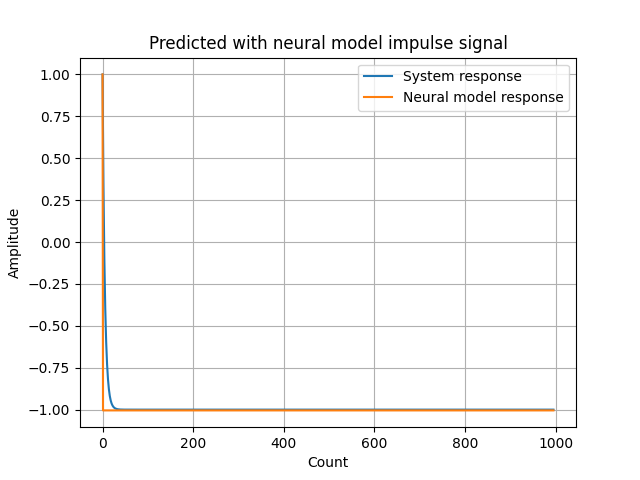
\includegraphics[width=1\linewidth]{body/images/Predicted-with-neural-model-impulse-signal.png}
	\caption{Отклик системы и смоделированный отклик нейросети, обученной на импульсном воздействии}
	\label{fig:20}
\end{figure}

На графике (Рис. \ref{fig:20}) видно, что отклик, смоделированный нейросетевой моделью, отличается от отклика системы. Плавный переход отклика системы
заменяются резким перепадом значения смоделированного отклика. Это вызвано тем, что отклик системы представляет собой, по большей части,
константную прямую. Плавный переход стирается из-за разницы количества значений и остаётся один лишь пик, который и показывает собой импульсное воздействие


\subsubsection{Нормированное импульсное воздействие}

\begin{figure}[H]
	\centering
	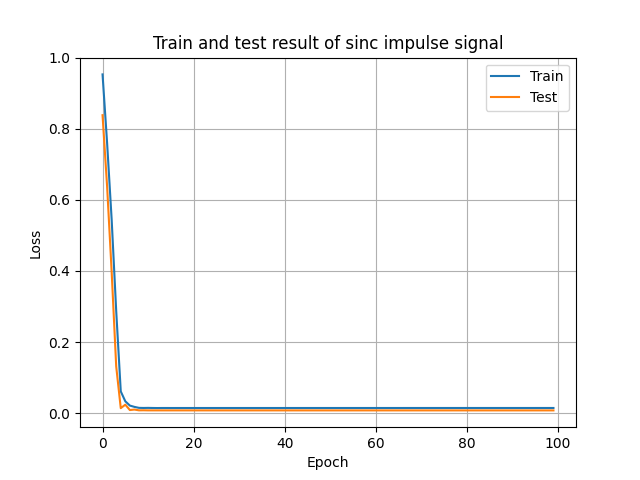
\includegraphics[width=1\linewidth]{body/images/Train-and-test-result-of-sinc-impulse-signal.png}
	\caption{Отклонение значений при тренировке и тестирования нейросети, обученной на нормированном импульсном воздействии}
	\label{fig:21}
\end{figure}

Мы видим график (Рис. \ref{fig:21}), схожий с обратной пропорциональностью, который опадает невероятно быстро.
По сути он практически повторяет собой график из предыдущего эксперимента с импульсным воздейтствием. Вывод к этому графику также
повторяется

\begin{figure}[H]
	\centering
	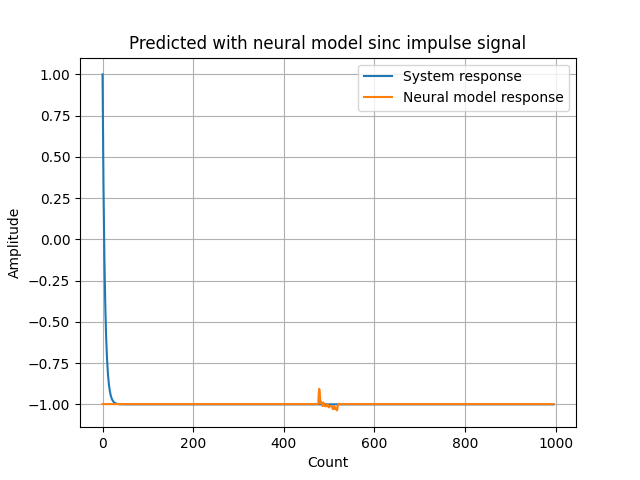
\includegraphics[width=1\linewidth]{body/images/Predicted-with-neural-model-sinc-impulse-signal.png}
	\caption{Отклик системы и смоделированный отклик нейросети, обученной на нормированном импульсном воздействии}
	\label{fig:22}
\end{figure}

На графике (Рис. \ref{fig:22}) видно, что отклик, смоделированный нейросетевой моделью, отличается от отклика системы. Он больше
похож на сигнал, поданный на вход системы. Для него характерна такая же центрация главного лепестка. Видны и следы лепестков поменьше: из-за
этого на нейросетевой модели и видна небольшая полоса нестабильности

\subsubsection{Меандр}

\begin{figure}[H]
	\centering
	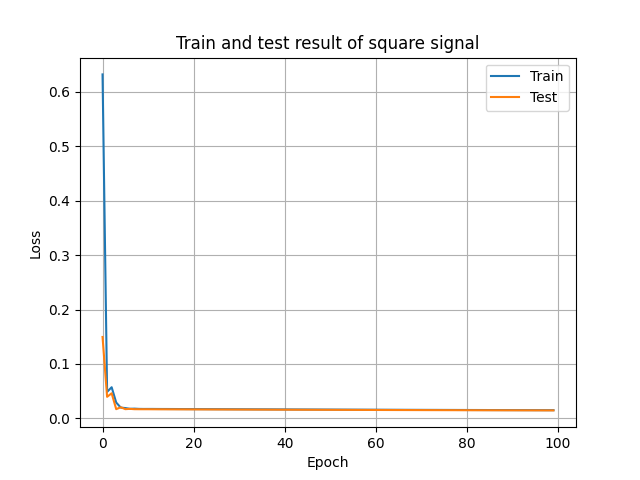
\includegraphics[width=1\linewidth]{body/images/Train-and-test-result-of-square-signal.png}
	\caption{Отклонение значений при тренировке и тестирования нейросети, обученной на меандре}
	\label{fig:23}
\end{figure}

На графике (Рис. \ref{fig:23}) некое замешательство на начальных эпохах. Это объясняется видом отклика системы, используемом для обучения нейросетевой 
модели. Края вершин меандра немного скруглены под влиянием линейного звена

\begin{figure}[H]
	\centering
	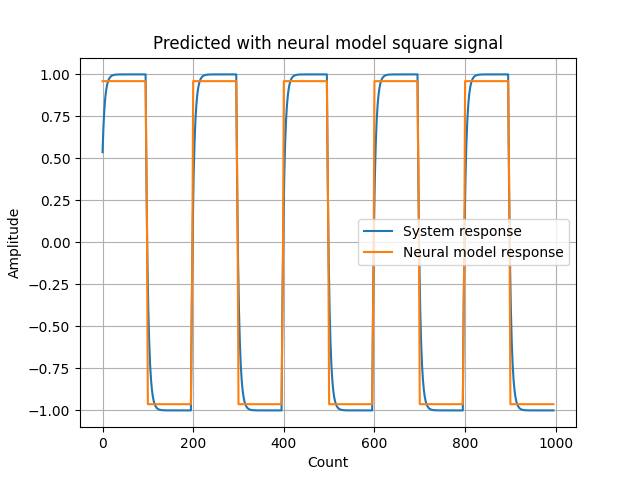
\includegraphics[width=1\linewidth]{body/images/Predicted-with-neural-model-square-signal.png}
	\caption{Отклик системы и смоделированный отклик нейросети, обученной на меандре}
	\label{fig:24}
\end{figure}

На смоделированном же отклике (Рис. \ref{fig:24}) мы видим практически чистый меандр.
Об этом уже говорилось выше. Как я считаю, так происходит из-за резких перепадов значений сигнала, которые напоминают собой
разрывы 1-го рода. Возможно из-за этого выполняется неполная идентичность модели

\subsubsection{Ступенчатое воздействие}

\begin{figure}[H]
	\centering
	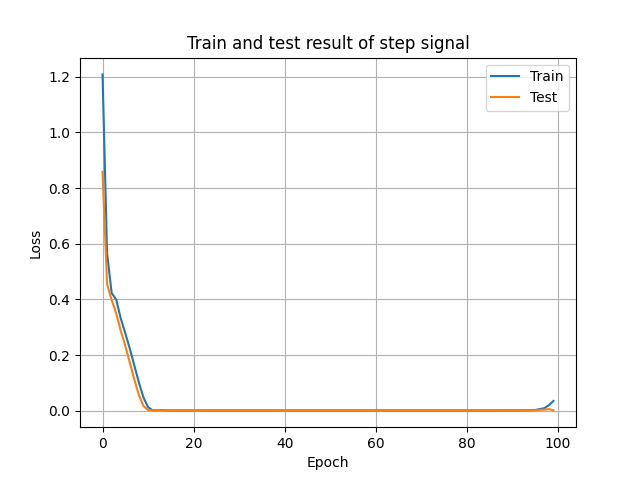
\includegraphics[width=0.7\linewidth]{body/images/Train-and-test-result-of-step-signal.png}
	\caption{Отклонение значений при тренировке и тестирования нейросети, обученной на ступенчатом воздействии}
	\label{fig:25}
\end{figure}

На графике (Рис. \ref{fig:25}) видно, что нейросетевая модель на начальных эпохах пытается найти зависимость между скруглением, обоснованным
начальными условиями и константной прямой, а далее между ней и резкой сменой значения. На 50-ой эпохе виден странный пик, который не поддаётся объяснению 

\begin{figure}[H]
	\centering
	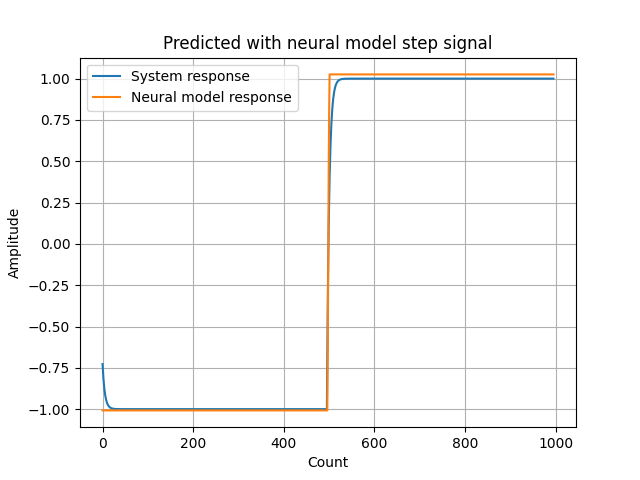
\includegraphics[width=0.7\linewidth]{body/images/Predicted-with-neural-model-step-signal.png}
	\caption{Отклик системы и смоделированный отклик нейросети, обученной на ступенчатом воздействии}
	\label{fig:26}
\end{figure}

Поскольку, как отмечалось выше, ступенчатое воздействие можно расценивать как меандра с большой скважностью, то и вывод будет здесь один и тот же

\subsection{Нейросетевая модель на общей выборке}

В этом пункте используется такая же методика, как и в предыдущем, за исключением того, что теперь
датасет формируется последовательно из всех сигналов кроме того, который мы хотим предсказать

В этом пункте мы рассмотрим только показательные сигналы: а именно моногармонический и меандр

\subsubsection{Моногармонический сигнал}

\begin{figure}[H]
	\centering
	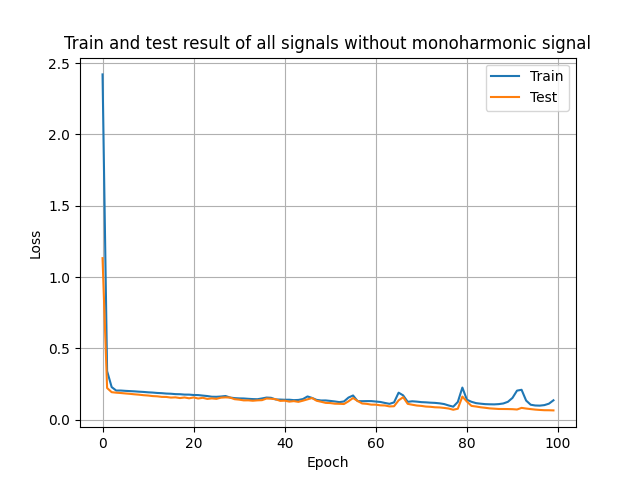
\includegraphics[width=0.7\linewidth]{body/images/Train-and-test-result-of-all-signals-without-monoharmonic-signal.png}
	\caption{Отклонение значений при тренировке и тестирования нейросети, обученной на общем датасете, не включая моногармонический сигнал}
	\label{fig:27}
\end{figure}

На графике (Рис. \ref{fig:27}) видно, на всех эпохах имеет затруднения с обучением. Это вызвано разнородностью сигналов и поиском зависимостей между ними.
Взглянув на отклонения тестовых значений мы видим, как график, по сравнению с тренировочными, начинает сглаживаться. С увеличением количества эпох возможно решение
проблемы с обучаемостью и пиками отклонений

\begin{figure}[H]
	\centering
	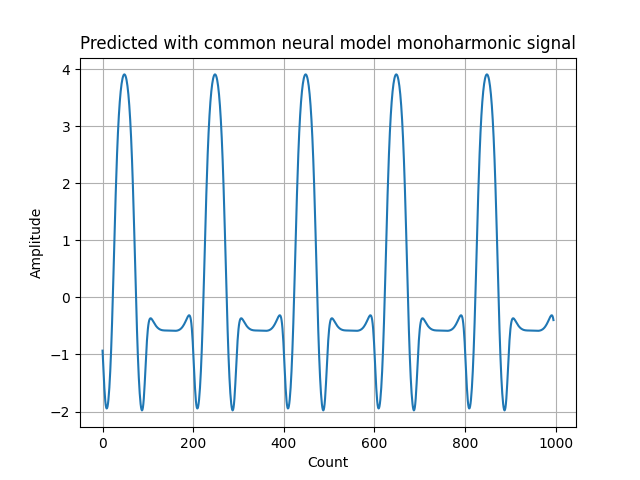
\includegraphics[width=0.6\linewidth]{body/images/Predicted-with-common-neural-model-monoharmonic-signal.png}
	\caption{Отклик системы и смоделированный отклик нейросети, обученной на общем датасете, не включая моногармонический сигнал}
	\label{fig:28}
\end{figure}

Рассматривая график смоделированного отклика (Рис. \ref{fig:28}), можно заметить, что он напоминает моногармонический сигнал, но лишь отдалённо. Как уже отмечалось выше,
это связано с разнородностью сигналов. В общем датасете присутствует только один периодический сигнал. Остальные же сигналы преобладаются и имеют больший диапазон
значений, в которых нет никакого отклонения. Поэтому на графике видны лепестки, но не видно, что бы они сохраняли форму моногармонического сигнала

\subsubsection{Меандр}

\begin{figure}[H]
	\centering
	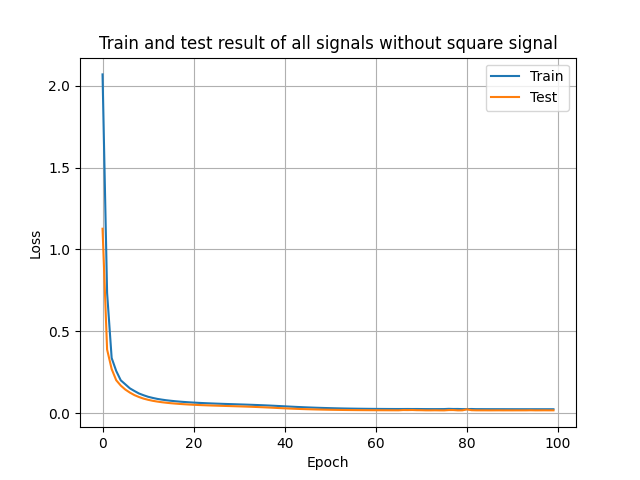
\includegraphics[width=0.6\linewidth]{body/images/Train-and-test-result-of-all-signals-without-square-signal.png}
	\caption{Отклонение значений при тренировке и тестирования нейросети, обученной на общем датасете, не включая моногармонический сигнал}
	\label{fig:29}
\end{figure}

На графике (Рис. \ref{fig:29}) видно, что в отличие от моногармонического сигнала обучение происходит плавно. Так происходит, потому что
меандр в обучающем датасете заменился на моногармонический сигнал, в котором преобладает скругленённость, нежели чем строгие прямые углы

\begin{figure}[H]
	\centering
	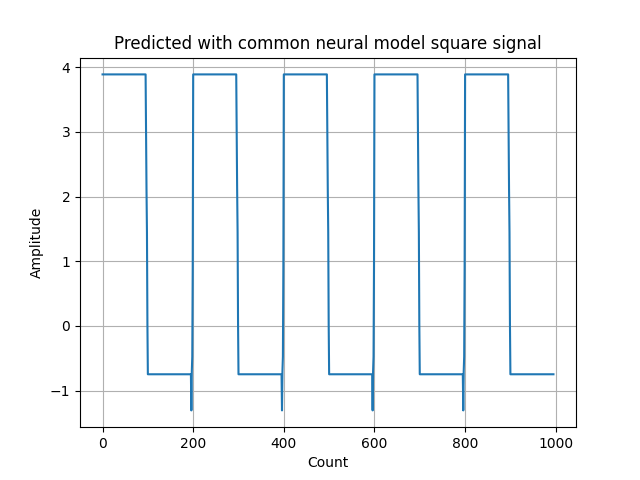
\includegraphics[width=0.7\linewidth]{body/images/Predicted-with-common-neural-model-square-signal.png}
	\caption{Отклик системы и смоделированный отклик нейросети, обученной на общем датасете, не включая моногармонический сигнал}
	\label{fig:30}
\end{figure}

Рассматривая график смоделированного отклика (Рис. \ref{fig:30}), можно сказать, что он практически полностью представляет собой меандр.
Из общей массы выбиваются только небольшие пики на лепестках меандра. Я полагаю, они вызваны всё тем же недостатком датасета: слишком большая часть
значений представляет собой последовательность значений без малейшего отклонения

\newpage

\subsection{Вывод}

В ходе работы была определна возможная структура исследуемого объекта. Империческим путём было выяснено присутствие нелинейного звена "Идеальное реле" и линейного звена.
В качестве нелинейных параметров используются: для положительного знака - $ c_1 = 4.9 $, а для отрицательного $ c_2 = 0.8 $.
В качестве линейного звена выступает апериодическое звено с параметрами: коэффициент усиления $ k = 0.9 $ и постоянной времени $ T = 0.25 $

Были изучены средства моделирования сигналов, модельный подход к вычислению вида системы. Были проделаны эксперименты с нейросетевой моделью, где был 
выявлен недостаток датасета из-за нехватки в нём большего разнообразия сигналов, а также нехватки периодических сигналов

